\expandafter\ifx\csname ifdraft\endcsname\relax
\documentclass[11pt]{article}
\usepackage[dvipdfmx]{graphicx}
\begin{document}
\fi

\section{はじめに}  
 %発表時にどのような意見が欲しいのか補足する
現在,コマンドとテレメトリを用いた衛星の故障箇所の特定を
支援する手法を検討している.\\
以下の章では,まず研究背景として地上試験におけるリスク分析の不十分さ及び,
不具合原因仮説の検証を支援する研究が十分に行われていないことを述べ,次にそれを踏まえた
研究目的に関して述べる.
また,提案手法の章では,不具合分析のアルゴリズム,
使用するモデルに関して述べ,そのモデルを用いた仮説検証のための
コマンド及び確認事項の探索方法,人がコマンド選択をする際に必要な
評価指標に関して説明する.
最後に,簡易衛星モデルを用いた実践例を示し,今後の方針について述べる.

\section{研究背景} 
\subsection{超小型衛星の信頼性の低さ}

超小型衛星の開発が大学や小企業の中で盛んになってきている.
これまでは教育目的が主であったが,商用利用や革新的なミッションへの応用も
増えてきている\cite{Langer2016}.
一方で現状の超小型衛星は中・大型衛星と比較して軌道上での不具合の確率は高く,
2002から2016の間に打ち上がった
270のCubesatのうち,139のミッションが失敗している\cite{Langer2016}.\\
これらの不具合は,大学衛星が宇宙環境での使用を保証されていない
民生部品を使用することも多いため,軌道上での部品の故障によって
発生すると考えられてきた.しかし,
実際には多くが設計や製造過程に起因する
不具合であることが知られている\cite{Venturini2017}.
軌道上での不具合の根本原因に対する調査(Figure \ref{fig:cause of failure})では,
民生部品の品質の不確定性が原因であったものはわずか17%であり,
それ以外の多くが設計や,地上試験の不足に起因するものである\cite{Venturini2017}.

%ここにできれば具体的な衛星の故障の例を持ってくれると良い
%論文で
\begin{figure}[H]
   \centering
      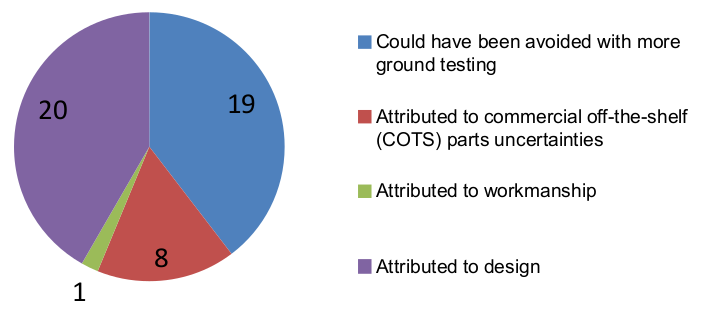
\includegraphics[height=4.5cm]{figure/cause_of_failure.png}
      \caption{故障原因に関するインタビュー結果\cite{Venturini2017}}
      \label{fig:cause of failure}
\end{figure}

%ここへのつながり
また,大学衛星が商用利用や革新的なミッションに
挑戦するためには,超小型衛星のメリットである
コストの低さを十分に確保しながら,
ほどよい信頼性を実現することが,重要であると考えられている\cite{SHIRASAKA2011}.\\
故障に設計や製造の不良が含まれていることを考えると,
超小型衛星の「ほどよい信頼性」の評価を行うためには,
従来用いられてきた
各コンポーネントごとの信頼度の組み合わせでは不十分である.
そこで,設計・製造・運用における
信頼度を加味した評価手法が提案されている\cite{SHIRASAKA2011}.
式(\ref{eq:Reliability})が示すように,この評価手法では
製造時の信頼性も重要な要素であると捉えられている.

\begin{equation}
   R_{sat} = R_{des} \times R_{fab} \times R_{comp} \times R_{op} \label{eq:Reliability}
\end{equation}
\begin{table}[H]
   \centering
      \begin{tabular}{cl} 
        $R_{sat}$ & 衛星の真の信頼度\\
        $R_{des}$ & 設計における信頼度\\
        $R_{fab}$ & 製造における信頼度\\
        $R_{comp}$ & 衛星の信頼度(従来の信頼度)\\
        $R_{op}$ & 運用における信頼度
      \end{tabular}
\end{table}

%もうちょいちゃんと考える
\subsection{地上試験における問題}
以上で示したように,不具合の多くが設計,製造などに起因している
という問題がある.
一方で,これは超小型衛星開発のみに限られたことではなく,
中・大型衛星においても大きな問題となっている.
軌道上故障データを分析した結果\cite{SAITO2011}(Figure \ref{fig:error tyoe})
によると,軌道上で
偶発的に発生した故障はわずか11%であり,それ以外は設計,製造などの開発
活動に起因するものであることがわかっている.\\
また,軌道上で発生した不具合が地上試験で
発現しなかった,または発見できなかった原因が以下の
Figure \ref{fig:error cause}のように知られている.
試験設備の不足によるものや,故障発見までの
時間が長く試験で発見することが現実的で無いものに関しては,
コストとリソースの面から試験による対策では限界がある.
一方で,試験モードの不備や,発現していたのにもかかわらず
発見できなかった不具合に関しては
試験に対する習熟度が不足していること,
不具合・リスクの分析が不十分であることが推測される\cite{SAITO2011}.

\begin{figure}[H]
   \centering
      \begin{tabular}{c}
         \begin{minipage}{0.50\hsize}
         \centering
         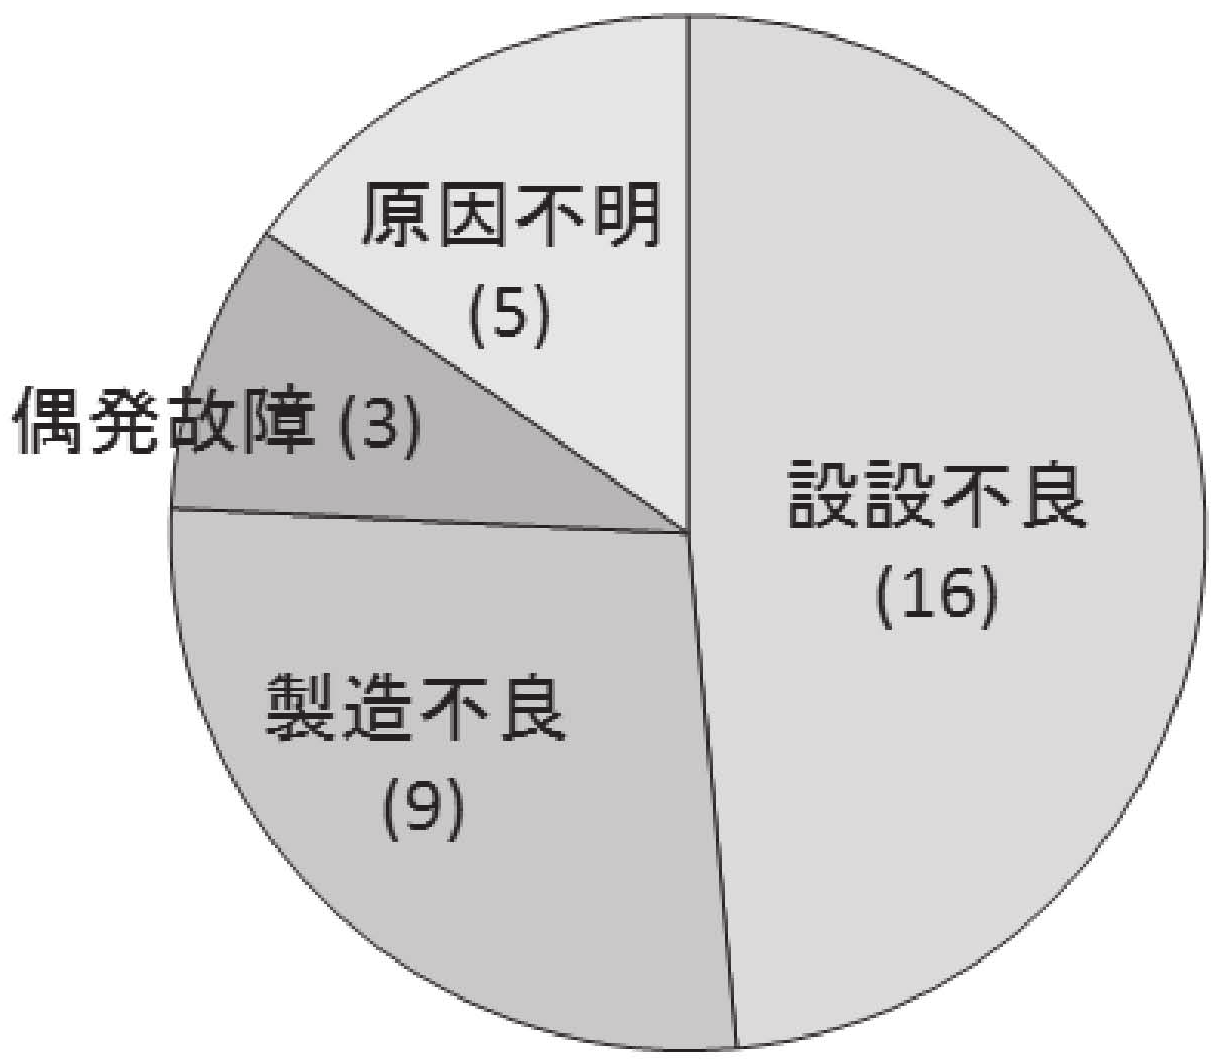
\includegraphics[width=5.5cm]{figure/on_orbit_error_tyoe.png}
            \caption{軌道上故障の原因類型の分布\cite{SAITO2011}}
            \label{fig:error tyoe}
         \end{minipage}
         \begin{minipage}{0.50\hsize}
         \centering
         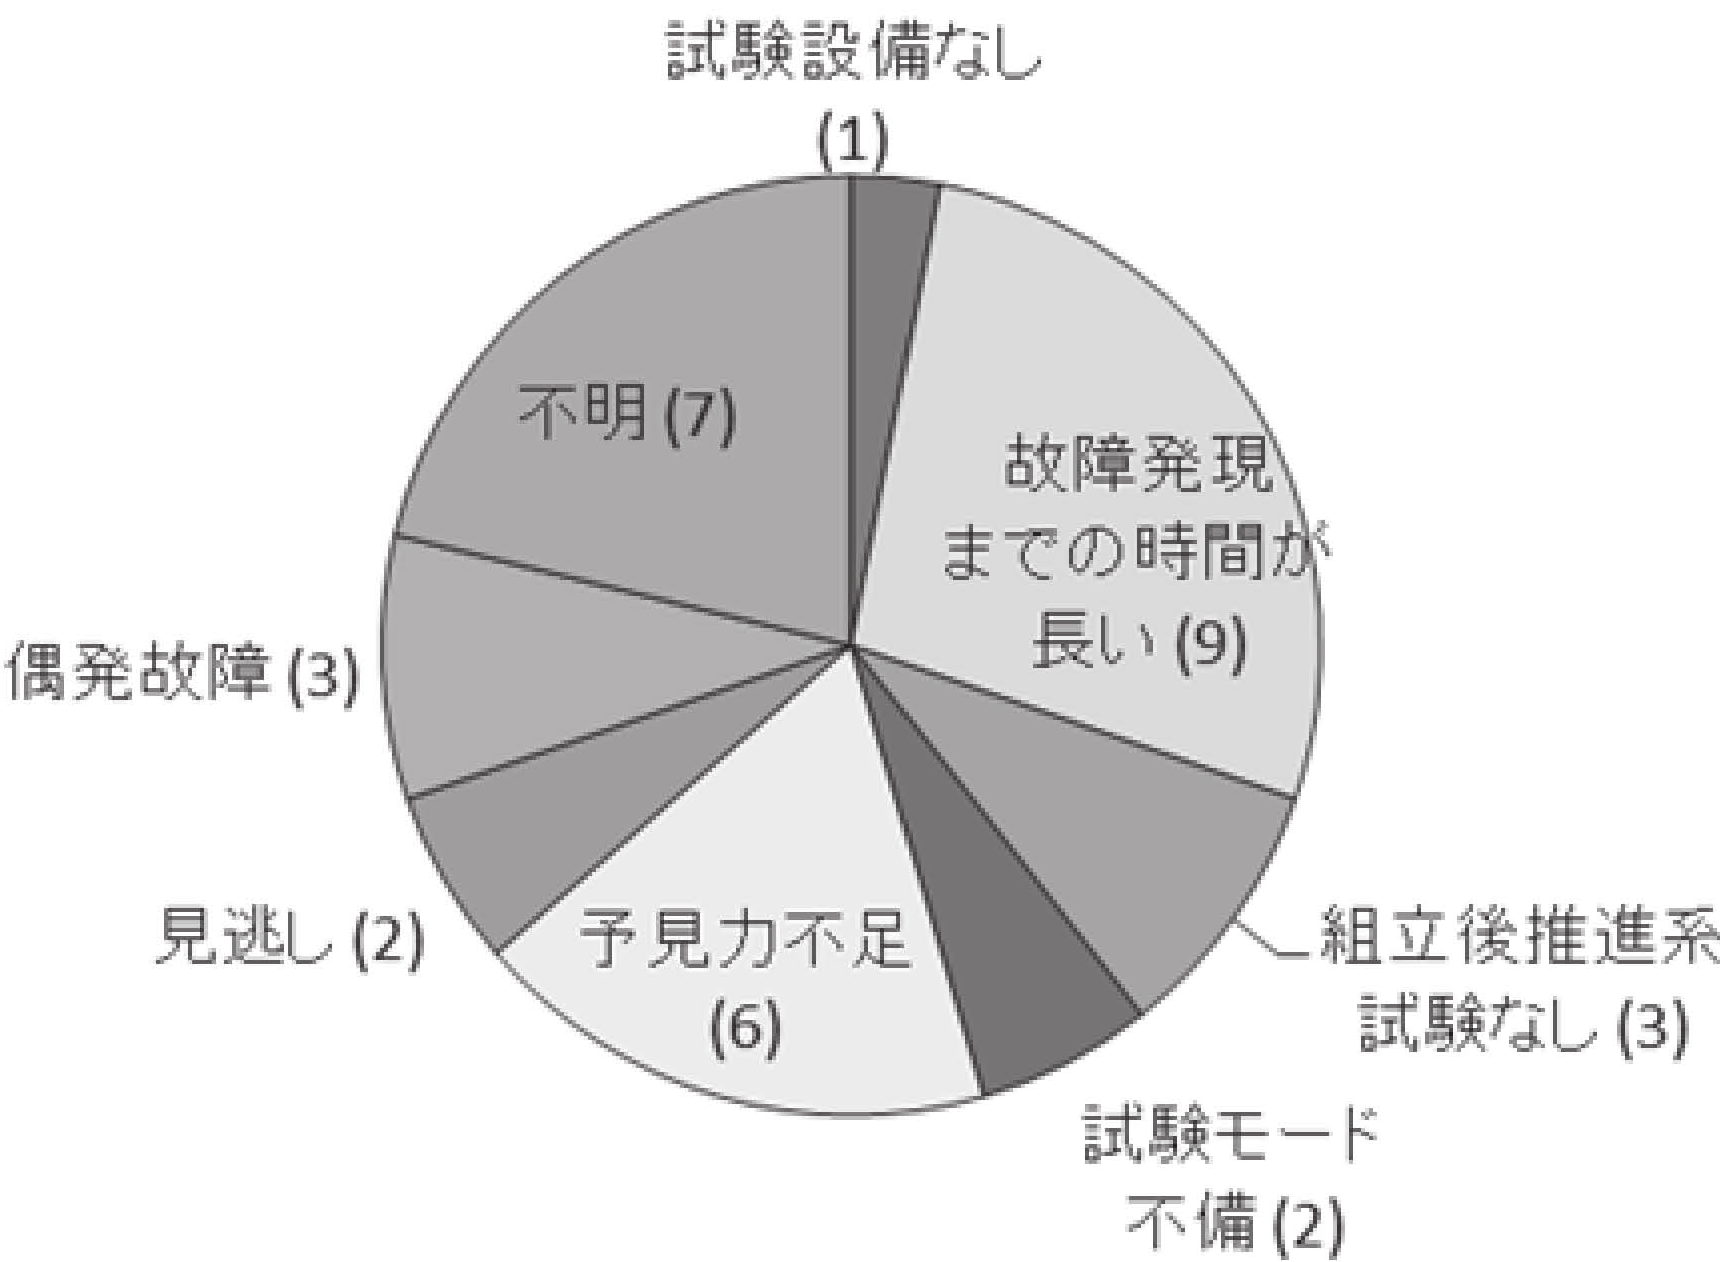
\includegraphics[height=5.5cm]{figure/not_found_error_seeds.png}
            \caption{軌道上故障の要因を地上で発見できなかった原因類型の分布\cite{SAITO2011}}
            \label{fig:error cause}
         \end{minipage}
      \end{tabular}  
\end{figure}

%ここの流れを見直す.根拠資料
\subsection{不具合原因特定の難しさ}
以上のように,衛星の不具合及びリスク分析を,地上試験で十分に
行うことができていないという現状がある.\\
その原因を具体的に示すため,以下に人間による不具合原因分析の大まかな流れを示す.
\begin{enumerate}[1)]
   \item 不具合が起きた際の衛星の状態を保存し記録に残す. 
   \item テレメトリから考えられる故障原因の候補を洗い出す.
   \item それらの故障の中でテレメトリから分かる情報を元に候補を棄却していく.
   \item 更に切り分けが必要な場合はコマンドを送り,
   それにに対するテレメトリの挙動によって判断するという作業を繰り返す.
   \item 判断できない場合は,コンポーネントを取り出し直接確認を行う.
\end{enumerate}
上の流れを元に
分析が不十分になっている原因を考える.まず,2)の故障原因の候補
の洗い出しを網羅的に行うことの難しさがある.
組み上げ状態の衛星から得られる情報はテレメトリのみである.
この際,衛星の内部状態を理解し,テレメトリから現在の衛星の状態
を想像することができなければ,十分に不具合原因の候補を洗い出すことはできない.\\
本研究室の過去プロジェクト(PRISM)を対象にした研究では,
事前に想定していた故障モードの粒度は,
%ここの記述も微妙なので変更する
山口ら\cite{Yamaguchi2014}がモデルを用いて洗い出したものと比較して,
不十分であるという結果も出ている.
このように,人による故障モードの洗い出しは思いつきによるものなので,
考えが及んでいないことが多い.

また,分析が不十分になっているもう一つの原因として,
3),4)の故障原因の切り分け作業の難しさもある.
超小型衛星は内部状態が複雑に絡み合っており,一つの不具合に対して
非常に多くの故障候補が洗い出されることが想像できる.
%切り分けを行うためのコマンドを探すのが難しい
そのため,多くの故障候補の中から切り分けを行い,最終的な故障を
特定するという作業は多くの知識と労力を必要とする作業である.
また,実ミッションで使用するコマンドとテレメトリは膨大な数であるため,
その中から切り分けを行うための情報を選択し,仮説の検証を行う作業は
無駄やヒューマンエラーを生むきっかけとなる.
検証作業の際,未熟な運用者が不具合原因特定のために誤った%ここの表現改める
コマンドを送信してしまうと,
衛星の生存を脅かす可能性がある.このため,不具合原因特定を行う際には
そのコマンドが”安全”なのかという点も非常に重要となる.

%切り分け作業の難しさもだが,先行研究の事例を示し,故障候補の洗い出しに関しては
%広く検討されていることを述べて,自分はこちら側をやるという方向で示せばいいのでは?

%それはそうだが,下の流れを作るためには用途に応じてコマンド選択の指標が変わることを説明したい

\subsection{不具合分析関連研究}
上述のように,不具合原因の洗い出し
が網羅的にできていないこと,コマンドとテレメトリを用いて
原因特定を行う過程が知識依存になっていること
が,不具合分析が不十分になっている原因の一つであった.%一つでないが
これらの課題に対して,古くから%古くから???
不具合分析システムの研究が盛んに行われている.
以下のTable \ref{tab:previous_research}に,モデルベースで
機械などを対象にした不具合分析,故障診断を行う手法に関してまとめた.
%比較軸が微妙過ぎる
\begin{table}[H]
   \centering
   \caption{不具合分析手法の比較}
   \label{tab:previous_research}
      \begin{tabular}{cccccc} \hline%もう少し示し方を考える.
         手法&故障網羅性&手法の目的%&モデル複雑度%専門家の知識が必要という点で?
         \\ \hline
         GDE&低&故障仮説生成%&低
         \\ %見てないし無くてもいいかも
         GDE+\cite{Struss1989}&中&故障仮説生成%&中
         \\
         網状故障解析\cite{Yamaguchi2014}&中&異常モード洗い出し%&高
         \\
         故障オントロジー\cite{Kitamura1999}&高&故障仮説生成%&高
         \\
         本手法&中&故障箇所特定%&中
         \\ \hline
      \end{tabular}
\end{table}
%ここで本手法を出すのは適切なのか?何か分からんくない?
%モデル複雑度が比較の指標になるのか?
%モデルベースで行う不具合分析手法として一般的なものは
故障仮説生成の研究に関しては,
機器の正常時のモデルだけでなく,故障時モデルを組み込んだもの\cite{Struss1989}や,
オントロジーを用いてプロセスのつながりまでモデル化したもの\cite{Yamaguchi2014},
異常伝播事象までモデル化して階層的な推論を行うもの\cite{Kitamura1999}などが
%不具合原因である機器の故障の原因などを探索可能にしたものなどが
あり,網羅的に故障候補を洗い出すために広く取り組まれている.
一方で,來村ら\cite{Kitamura1999}が効率の良い検証方法に関しては
今後の課題として言及しているように,故障仮説の検証に取り組んだものは少ない.
%衛星における不具合診断では,以上で述べたように検証段階に多くの問題が山積している.


\expandafter\ifx\csname ifdraft\endcsname\relax
\end{document}
\fi